\documentclass[12pt, a4paper, oneside]{ctexart}
\usepackage{geometry}
\usepackage{graphicx}
\usepackage{epstopdf}
\usepackage{listings}
\usepackage[dvipsnames]{xcolor}
\geometry{a4paper, scale=0.8}
\pagestyle{plain}

\ctexset{
    section={
        name = {,、},
        number = {\chinese{section}},
        format = \heiti\raggedright\zihao{3},
        aftername = 
    },
    subsection={
        name = {,、},
        number = {\arabic{subsection}},
        format = \heiti\raggedright\zihao{-3},
        aftername = 
    },
    subsubsection={
        name = {,、},
        number = {\arabic{subsection}.\arabic{subsubsection}},
        format = \heiti\raggedright\zihao{4},
        aftername = 
    }
}
\lstset{
 columns=fixed,       
 numbers=left,                                        
 numberstyle=\tiny\color{gray},                       
 frame=none,                                          
 backgroundcolor=\color[RGB]{245,245,244},            
 keywordstyle=\color[RGB]{40,40,255},                 
 numberstyle=\footnotesize\color{darkgray},          
 commentstyle=\it\color[RGB]{0,96,96},                
 stringstyle=\rmfamily\slshape\color[RGB]{128,0,0},   
 showstringspaces=false,                              
 language=c++,                                        
}


\title{并行程序设计实验:CPU架构编程}
\date{}

\begin{document}

\maketitle
Github仓库中包含算法的C++代码,数据处理和图像绘制的Python代码,实验报告的Latex源文件,实验时的部分
截图。地址:https://github.com/Yifan-Guan/Parallel-lab-1-CPU-programming.git
\section{N阶方阵与向量内积}
\subsection{算法设计}
\subsubsection{平凡算法}
逐列访问矩阵元素,一步外循环得到一个内积。
\begin{lstlisting}
void inner_product(int n, int* a, int** b, int* s)
{
	for (int i = 0; i < n; i++) {
		s[i] = 0;
		for (int j = 0; j < n; j++) {
			s[i] += a[i] * b[i][j];
		}
	}
}
\end{lstlisting}
\subsubsection{cache优化算法}
逐行访问矩阵元素,一步外循环只会得到内积的一个累加项。
\begin{lstlisting}
void inner_product(int n, int* a, int** b, int* s)
{
    for (int i = 0; i < n; i++) {
        s[i] = 0;
    }
    for (int j = 0; j < n; j++) {
        for (int i = 0; i < n; i++) {
            s[i] += a[i] * b[j][i];
        }
    }
}
\end{lstlisting}
\subsection{编程实现}
Arm平台:WSL(2.4.13.0)Ubuntu(22.04.5 LTS)系统下使用aarch64-linux-gnu-g++
((Ubuntu 11.4.0-1ubuntu1~22.04) 11.4.0)交叉编译,在qemu-aarch64
(6.2.0 (Debian 1:6.2+dfsg-2ubuntu6.25))上执行。

x64平台:WSL(2.4.13.0)Ubuntu(22.04.5 LTS)系统下使用g++ (Ubuntu 11.4.0-1ubuntu1~22.04) 11.4.0
编译执行。
\subsection{性能测试}
测试数据中,向量a:$a_i = i^2$,矩阵b:$b_{ij} = i + j$,问题规模迭代次数取100(每迭代一次,n增加10),
运行时间使用gettimeofday()函数获取。在arm平台上的测试结果与在x64平台上的测试结果分别绘制为折线图
\ref{product_arm}和折线图\ref{product_x64}。
\begin{figure}[ht]
    \flushleft
    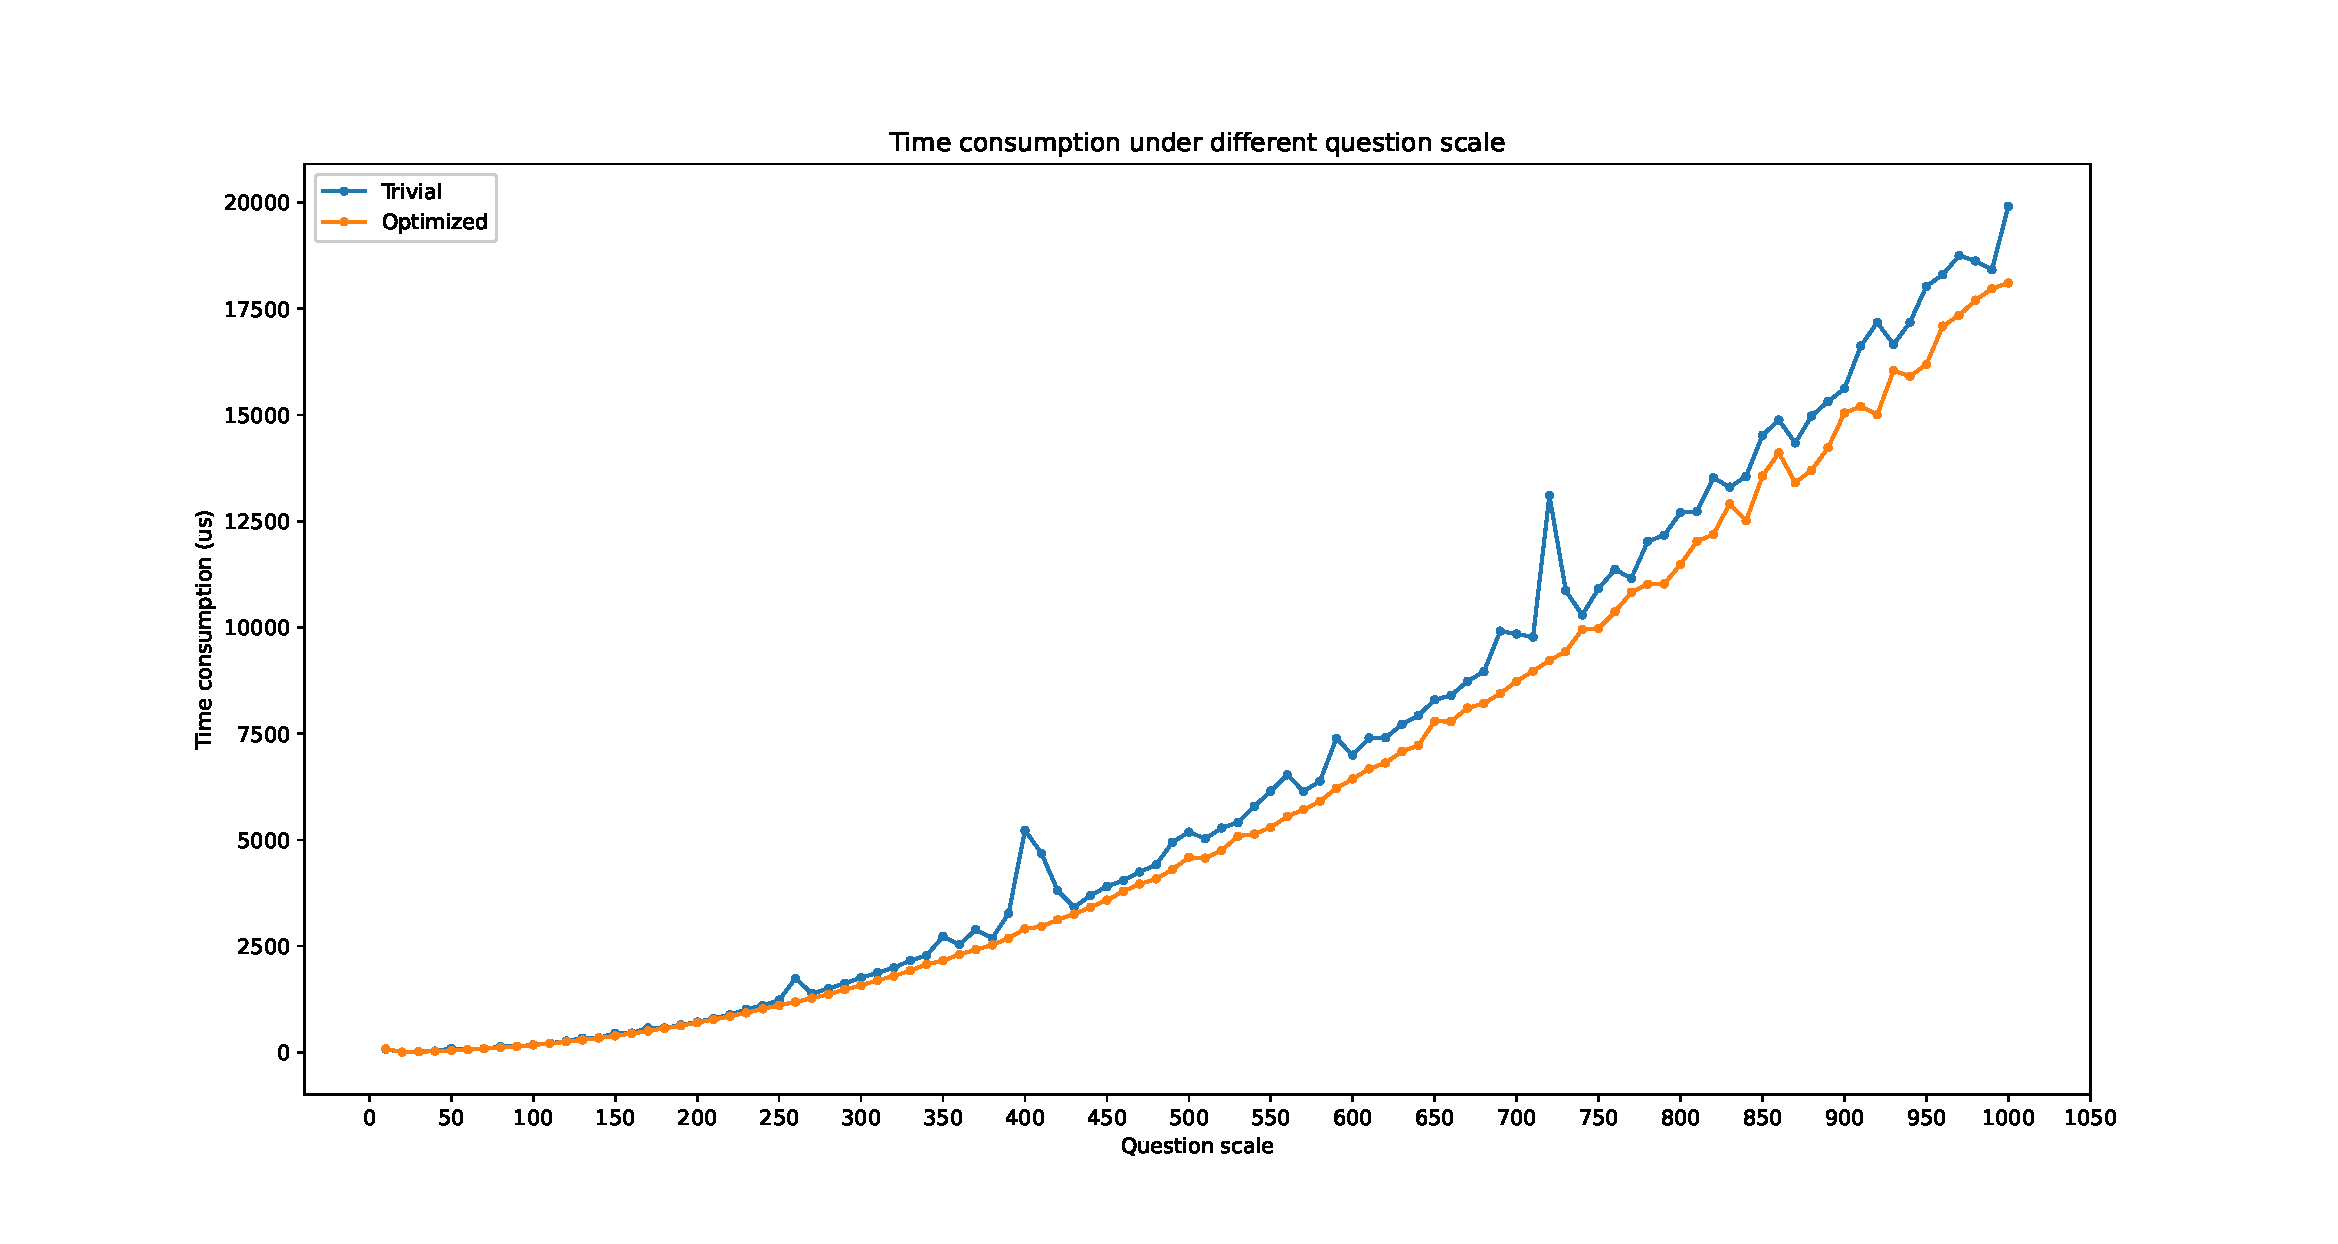
\includegraphics[scale = 0.5]{./picture/product_arm.eps}
    \caption{Product time consumption of arm}
    \label{product_arm}
\end{figure}
\begin{figure}[htbp]
    \flushleft
    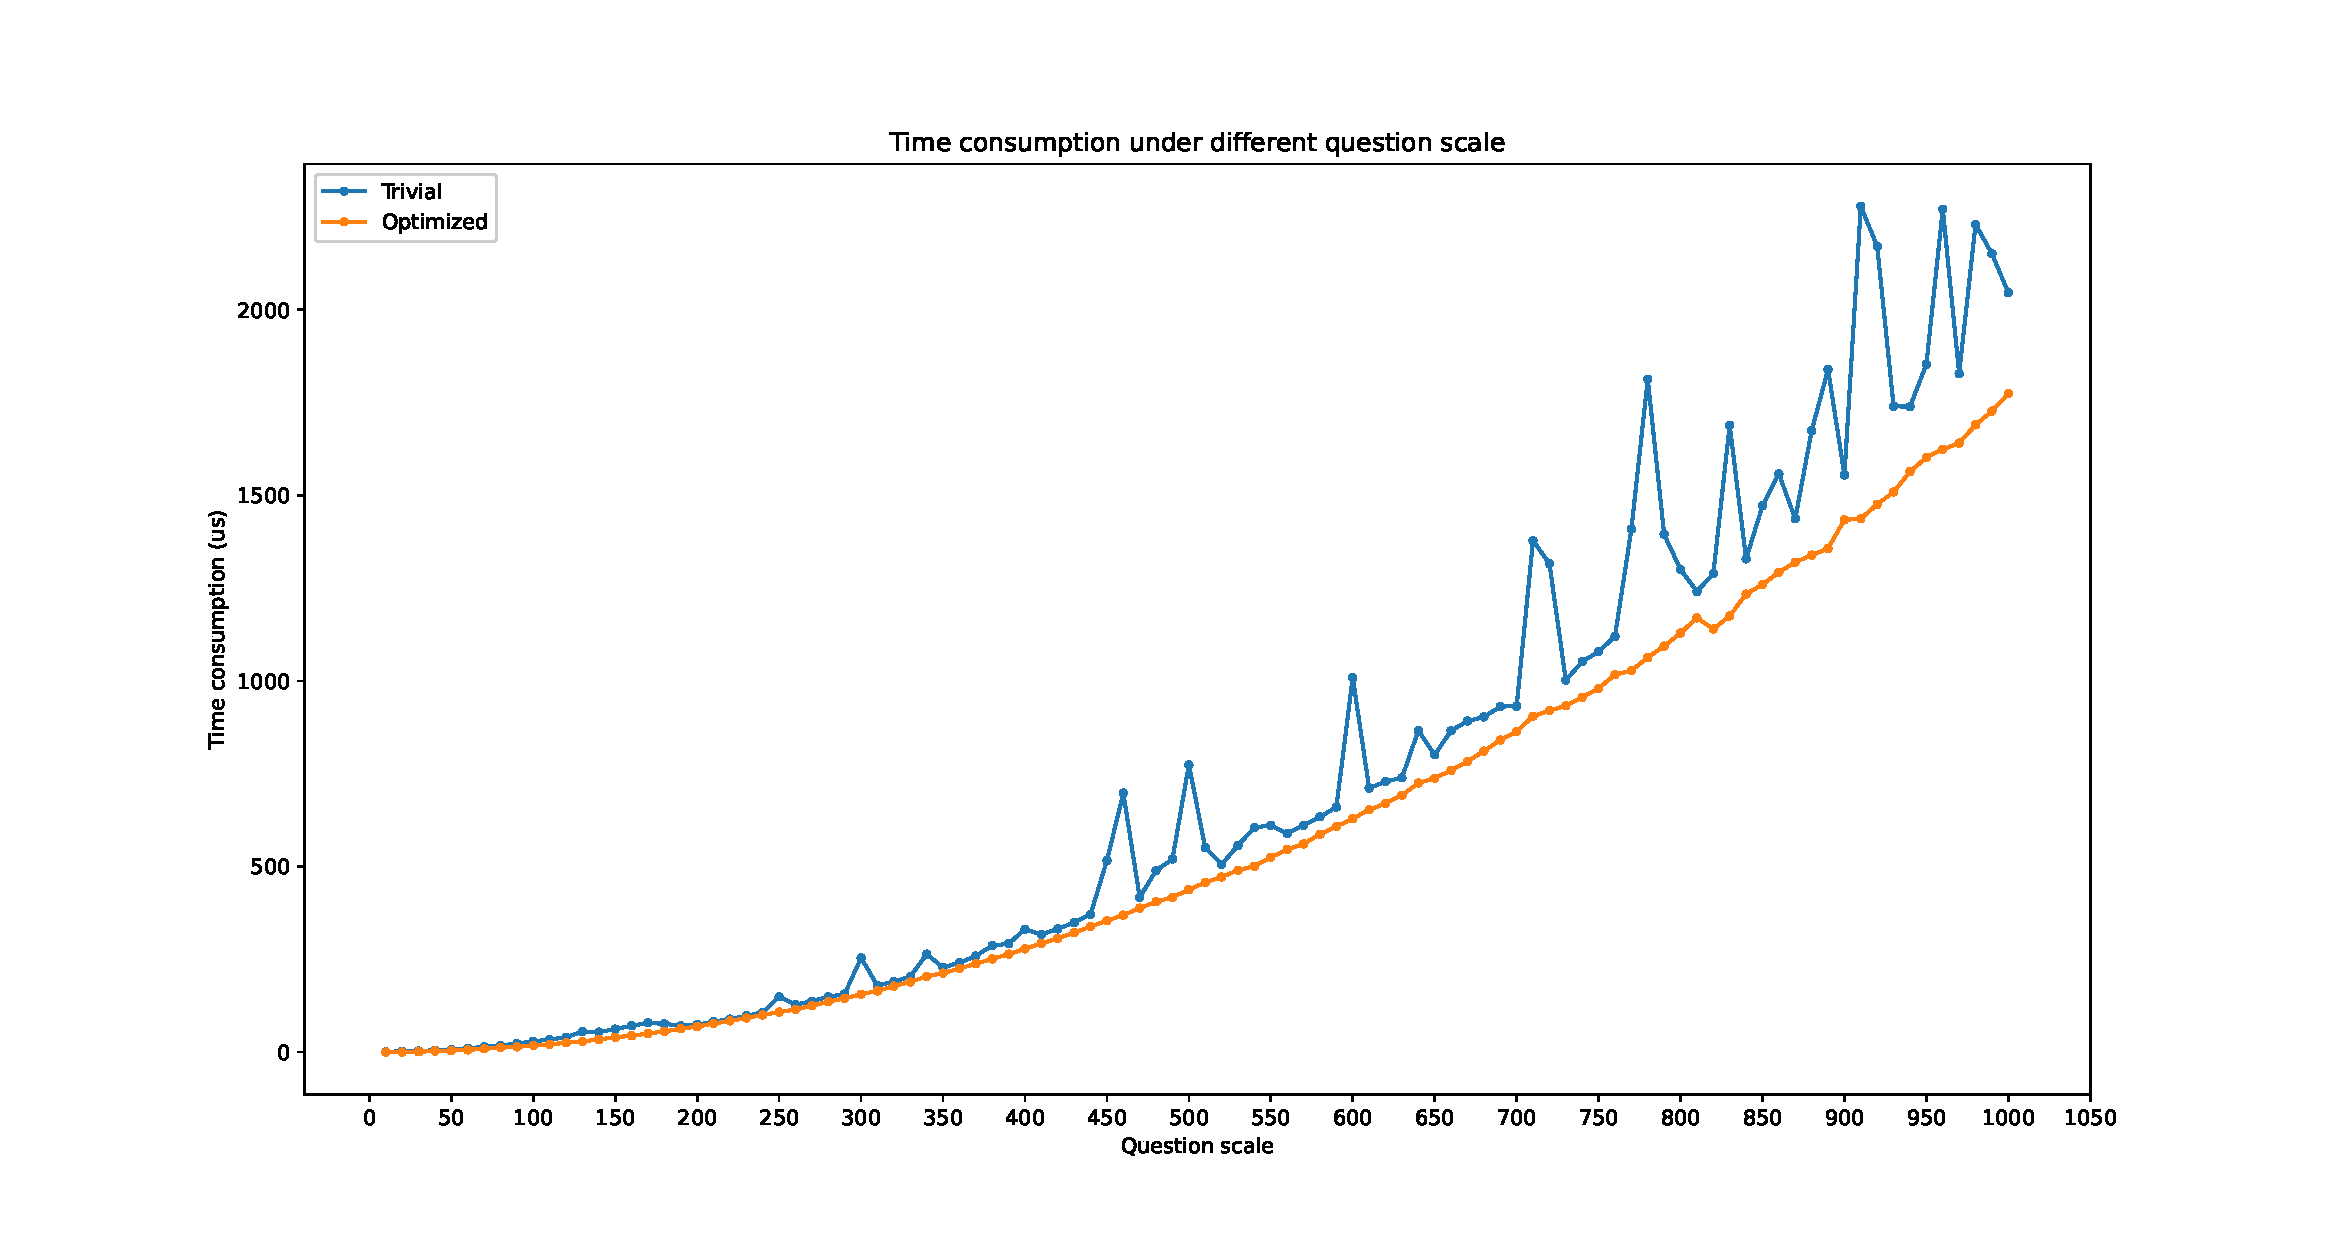
\includegraphics[scale = 0.5]{./picture/product_x64.eps}
    \caption{Product time consumption of x64}
    \label{product_x64}
\end{figure}
\subsection{profilling}
x64平台,WSL(2.4.13.0)Ubuntu(22.04.5 LTS)系统下使用perf(5.15.178)分别对程序运行时的Cache load,
Cache load miss, Cache prefetches指标进行分析,参数设置与上一节相同。得到结果绘制为表格\ref{product_perf}。
针对perf的分析报告,使用hotspot(1.3.0)绘制火焰图,分别为图\ref{pt_flame}和图\ref{po_flame}。
\begin{table}
\centering
\begin{tabular}{c c c c}
    \hline
    \multicolumn{4}{c}{Perf report of inner product} \\
    \hline
    \hline
    Program & L1-dcache-loads & L1-dcache-load-misses & L1-dcache-prefetches \\
    Trivial & 697614965 & 7722901 & 5268536 \\
    Optimized & 630400939 & 7577799 & 4972996 \\
    \hline
\end{tabular}
\caption{Perf分析结果}
\label{product_perf}
\end{table}
\begin{figure}[htbp]
    \centering
    \begin{minipage}{0.9\linewidth}
        \centering
        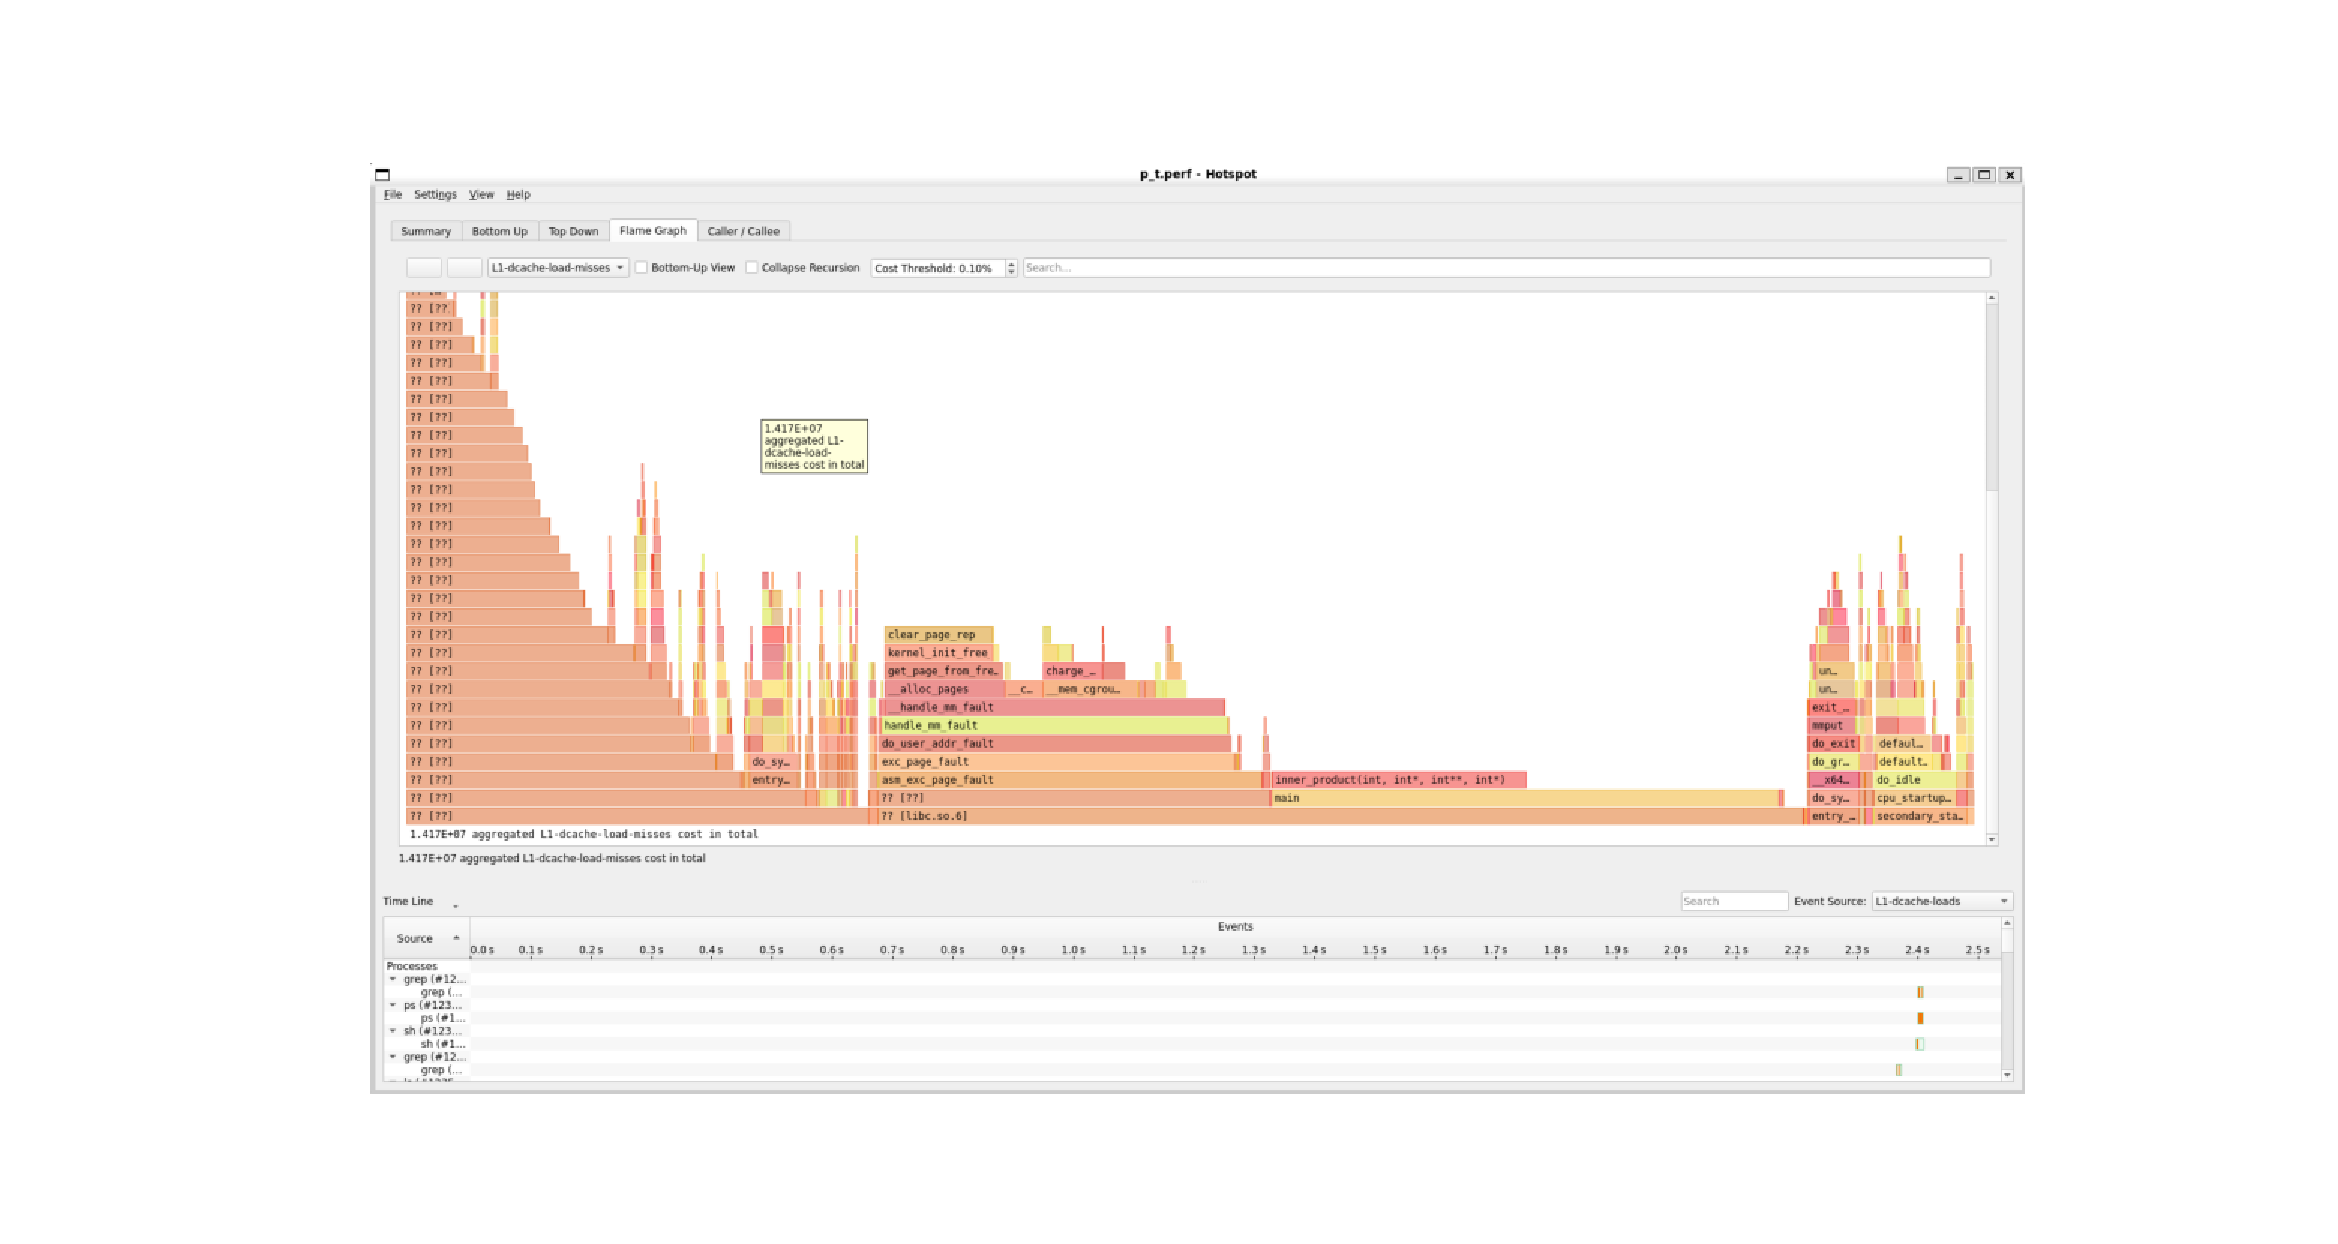
\includegraphics[scale = 0.4]{./picture/pt_flame.eps}
        \caption{Trivial算法的cache miss火焰图}
        \label{pt_flame}
    \end{minipage}
    \centering
    \begin{minipage}{0.9\linewidth}
        \centering
        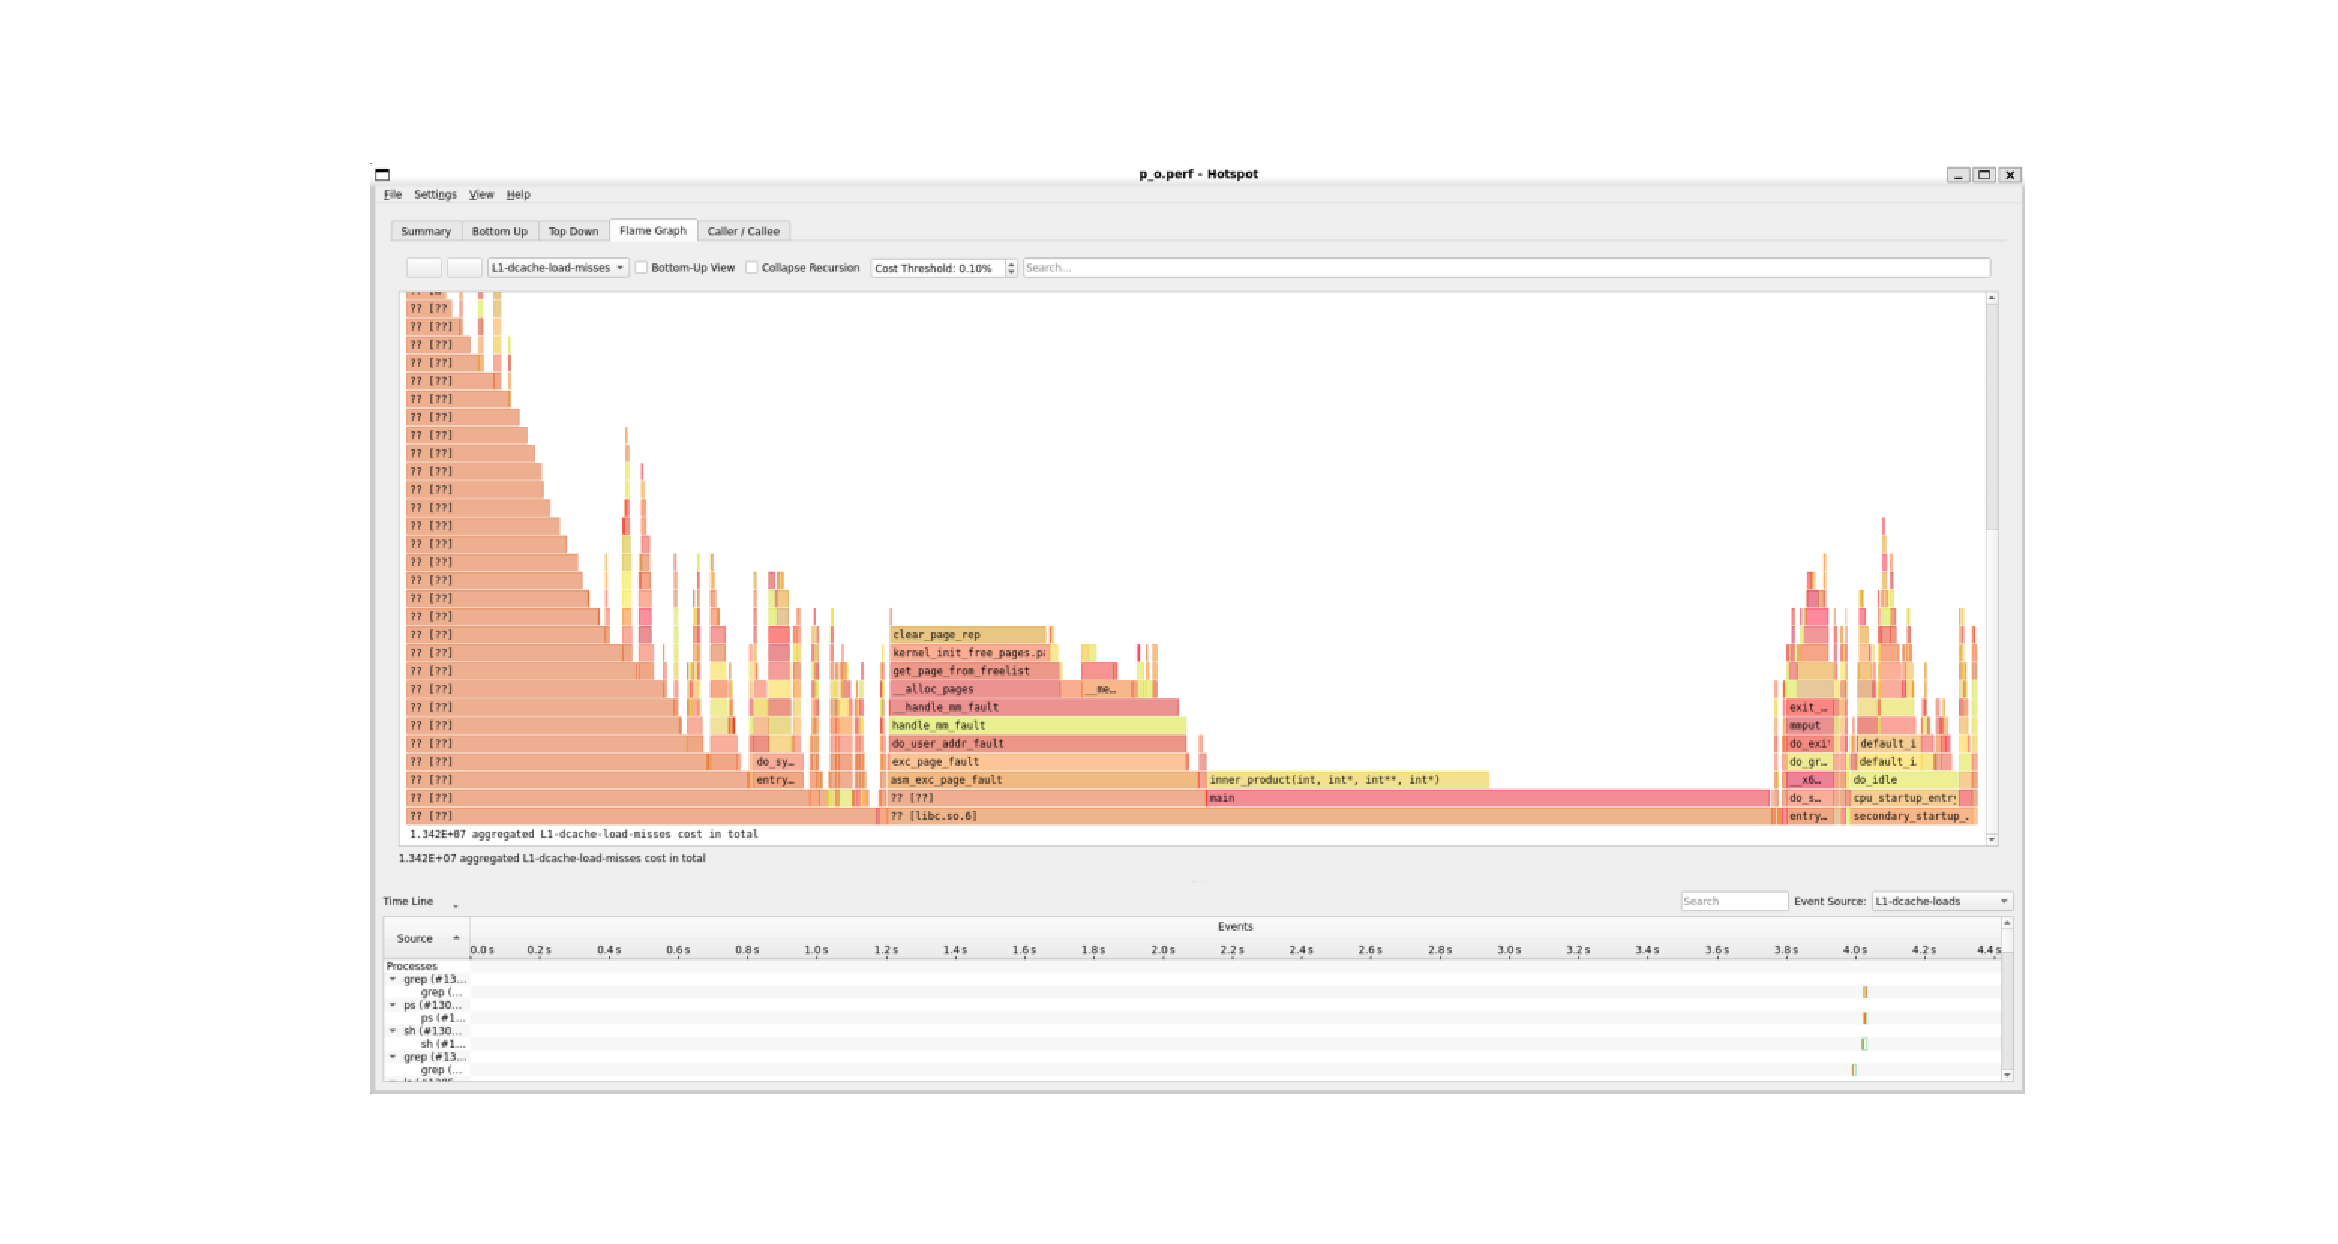
\includegraphics[scale = 0.4]{./picture/po_flame.eps}
        \caption{Optimized算法的cache miss火焰图}
        \label{po_flame}
    \end{minipage}
\end{figure}
\subsection{结果分析}
从折线图\ref{product_arm}和折线图\ref{product_x64}不难看出,使用了Cache优化算法运行时间显著降低,且
问题规模越大降低作用越明显。由于本实验中的arm环境是由WSL+qemu获得,性能上也显著弱于x64平台。由perf分析
结果表格\ref{product_perf}可知,Cache优化算法的Cache loads, Cache load misses, Cache prefetches
三项指标均低于平凡算法,Cache load missed火焰图也很好地佐证了这一点。

\section{N个数求和}
\subsection{算法设计}
\subsubsection{平凡算法}
链式算法,将所有元素累加得到最终结果。
\begin{lstlisting}
int sum(int n, int* a)
{
    int result = 0;
    for (int i = 0; i < n; i++) {
        result += a[i];
    }
    return result;
}
\end{lstlisting}
\subsubsection{超标量优化算法}
1、多链路算法,通过两个中间和变量,将循环次数减少一半。
\begin{lstlisting}
int sum(int n, int* a)
{
    int sum_1 = 0;
    int sum_2 = 0;
    for (int i = 0; i < n; i += 2) {
        sum_1 += a[i];
        sum_2 += a[i + 1];
    }
    return sum_1 + sum_2;
}
\end{lstlisting}
2、递归算法,加数从两端开始两两相加,得到中间结果后重复,直到得到最终结果。
\begin{lstlisting}
int sum(int n, int* a)
{
    if (n == 1) {
        return a[0];
    }
    else {
        for (int i = 0; i < n / 2; i++) {
            a[i] += a[n - 1 - i];
        }
        sum(n / 2, a);
    }
}
\end{lstlisting}
3、双循环算法,对于数列的前n/2项,有:$a_i = a_{i \times 2} + a_{i \times 2 + 2}$。这样每循环一次,
数列的长度减小一半,同时避免了递归算法对栈空间的大量需求。
\begin{lstlisting}
int sum(int n, int* a)
{
    for (int m = n; m > 1; m /= 2) {
        for (int i = 0; i < m / 2; i++) {
            a[i] = a[i * 2] + a[i * 2 + 1];
        }
    }
    return a[0];
}
\end{lstlisting}
\section{编程实现}
Arm平台:WSL(2.4.13.0)Ubuntu(22.04.5 LTS)系统下使用aarch64-linux-gnu-g++
((Ubuntu 11.4.0-1ubuntu1~22.04) 11.4.0)交叉编译,在qemu-aarch64
(6.2.0 (Debian 1:6.2+dfsg-2ubuntu6.25))上执行。

x64平台:WSL(2.4.13.0)Ubuntu(22.04.5 LTS)系统下使用g++ (Ubuntu 11.4.0-1ubuntu1~22.04) 11.4.0
编译执行。
\subsection{性能测试}
测试数据中,数列采用Fibonacci数列,即$a_i = a_{i - 1} + a_{i - 2}, i > 2, a_1 = a_2 = 1$。问题规模
迭代次数在arm平台上取20,在x64平台上取22(这是由于arm平台由wsl+qemu得到,性能低于x64平台),每迭代一次
问题规模增加一倍,确保值为2的幂。由于单次求和运算在问题规模较小时执行速度很快,所以得到的运行数据均是执行
100次的数据。性能测试时间使用gettimeofday()函数获取。在arm平台上的测试结果与在x64平台上的测试结果分别绘
制为折线图\ref{sum_arm}和折线图\ref{sum_x64}。
\begin{figure}[htbp]
    \centering
    \begin{minipage}{0.45\linewidth}
        \centering
        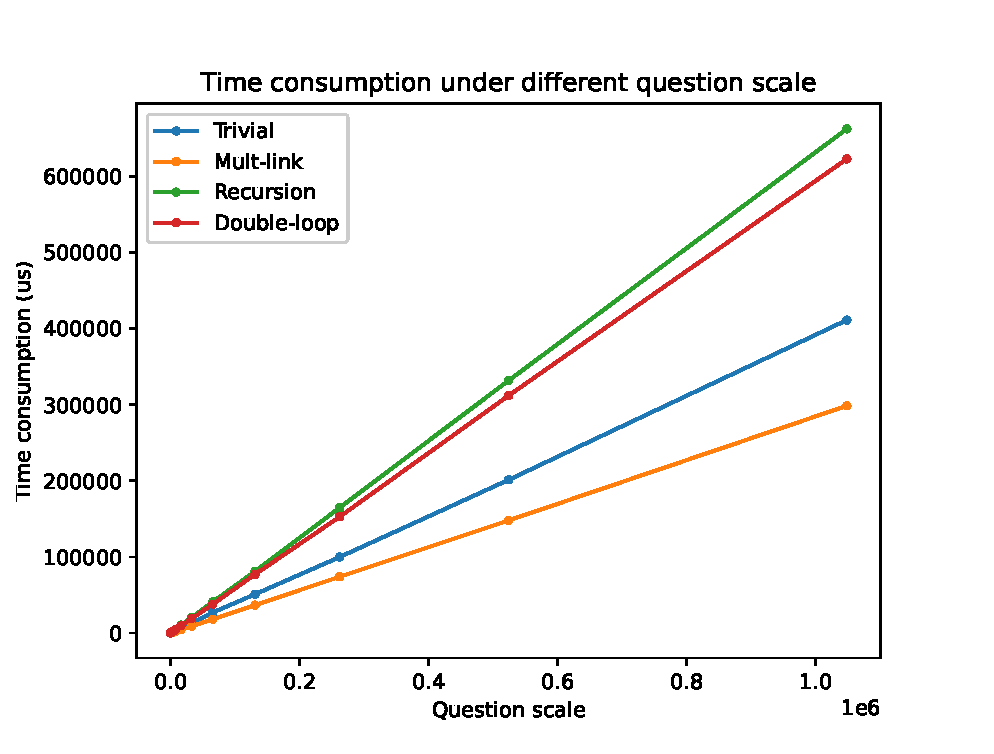
\includegraphics[scale = 0.5]{./picture/sum_arm_1.eps}
        \caption{$x = n$}
    \end{minipage}
    \centering
    \begin{minipage}{0.45\linewidth}
        \centering
        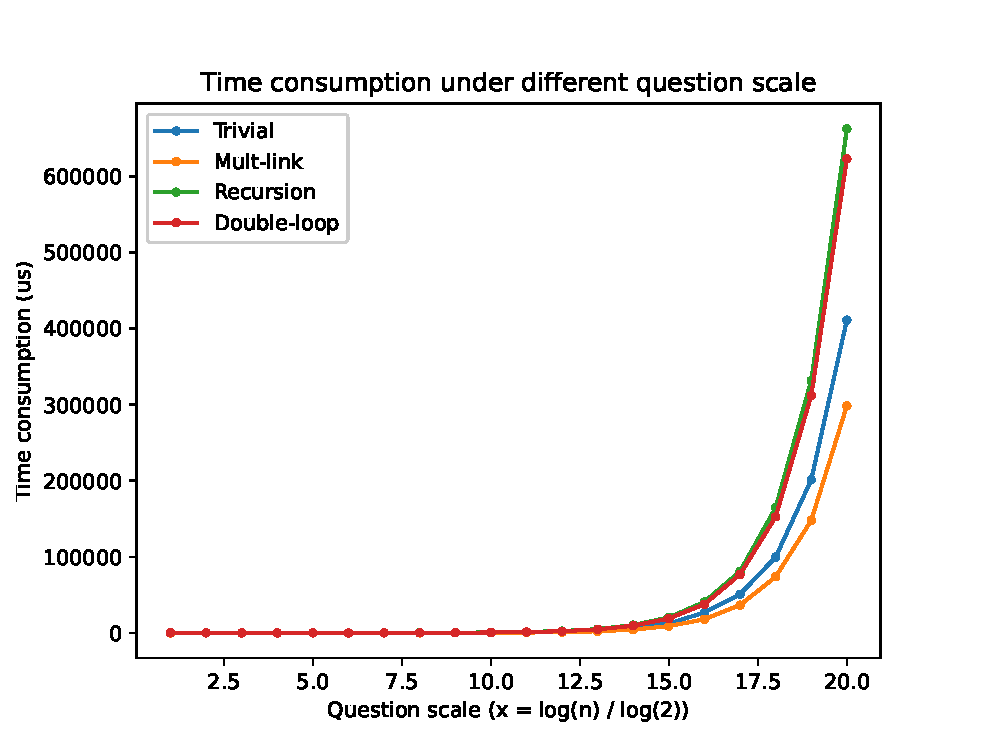
\includegraphics[scale = 0.5]{./picture/sum_arm_2.eps}
        \caption{$x = \log_2(n)$}
    \end{minipage}
    \caption{Sum time consumption of arm}
    \label{sum_arm}
\end{figure}
\begin{figure}[htbp]
    \centering
    \begin{minipage}{0.45\linewidth}
        \centering
        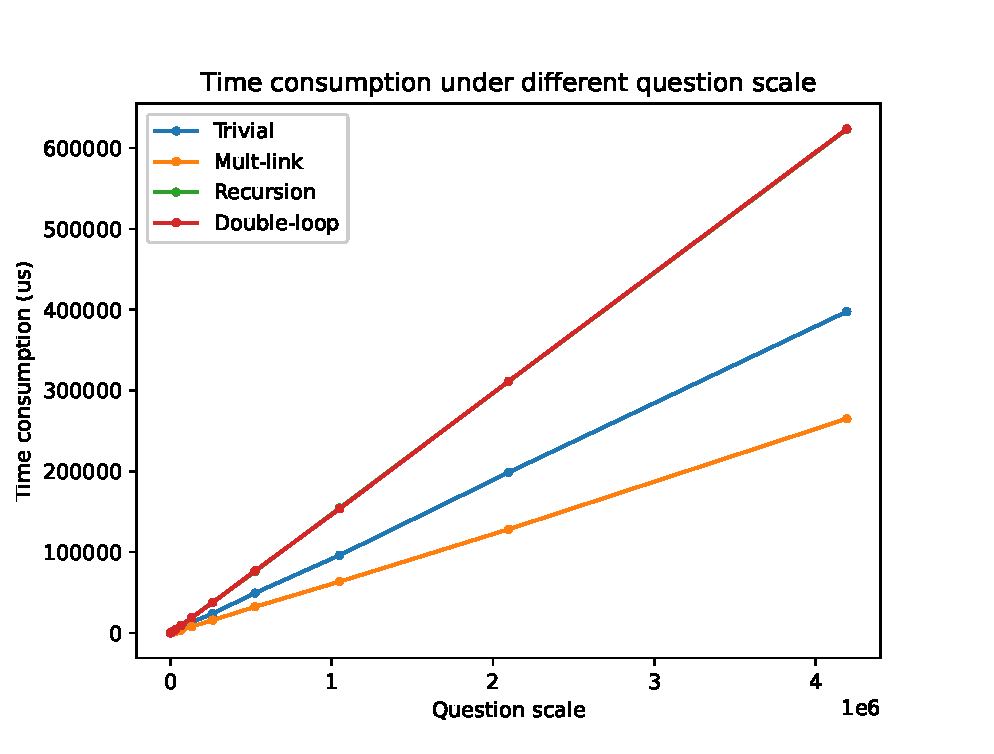
\includegraphics[scale = 0.5]{./picture/sum_x64_1.eps}
        \caption{$x = n$}
    \end{minipage}
    \centering
    \begin{minipage}{0.45\linewidth}
        \centering
        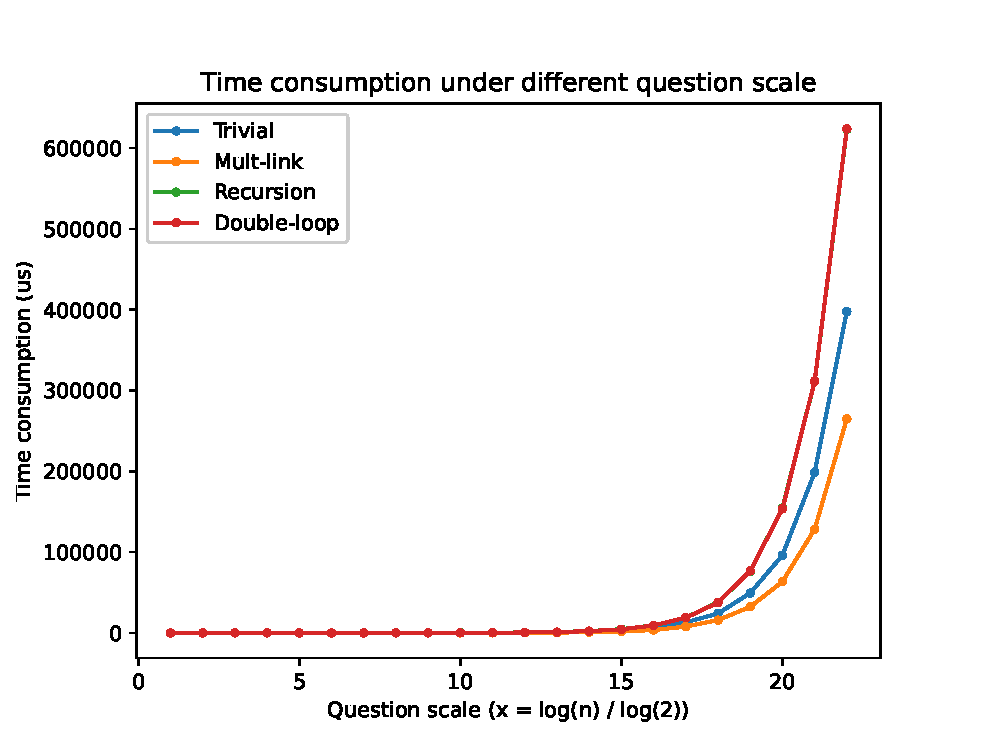
\includegraphics[scale = 0.5]{./picture/sum_x64_2.eps}
        \caption{$x = \log_2(n)$}
    \end{minipage}
    \caption{Sum time consumption of x64}
    \label{sum_x64}
\end{figure}
\section{profilling}
x64平台,WSL(2.4.13.0)Ubuntu(22.04.5 LTS)系统下使用perf(5.15.178)对平凡算法和三种优化算法运行
时的Instructions和Cycles进行分析,结果如表格\ref{sum_perf}所示。
\begin{table}
\centering
\begin{tabular}{c c c c c}
    \hline
    \multicolumn{4}{c}{Perf report of N-number summing} \\
    \hline
    \hline
    Program & Trivial & Mult-link & Resursion & Double-loop \\
    Instructions & 9449982541 & 8191702016 & 24550353073 & 25389039452 \\
    Cycles & 3401266727 & 2308548839 & 5238332656 & 5193907468 \\
    \hline
\end{tabular}
\caption{Pref分析结果}
\label{sum_perf}
\end{table}
\section{结果分析}
分析折线图\ref{sum_arm}与折线图\ref{sum_x64},优化算法中只有多链路算法的性能优于平凡算法,从perf
分析结果表\ref{sum_perf}可以看出,递归算法和双循环算法实际上对iterations和cycles的作用不减反增,
带来了更大的性能开销。

\end{document}